\documentclass[a4paper,10pt,oneside]{article}
\usepackage{graphicx}
\usepackage{color}
\usepackage{url}
\usepackage{subfigure}
\usepackage[utf8]{inputenc}
\usepackage[T1]{fontenc}
\usepackage{tgpagella}
%\usepackage[scale=0.9]{tgcursor}
%\usepackage[scale=0.9]{tgheros}
\usepackage{xstring}
\usepackage{wrapfig}

\newcommand{\myscale}{0.74}
\newcommand{\vect}[1]{\boldsymbol{#1}}
\newcommand{\code}[1]{\texttt{\StrSubstitute{#1}{.}{.\.}}}
\def\.{\discretionary{}{}{}}
\newcommand{\jmodule}[1]{\texttt{\textit{#1}}}

\setlength{\hoffset}{-1in} %left margin will be 0, as hoffset is by default 1inch
\setlength{\voffset}{-1in} %analogous voffset
\setlength{\oddsidemargin}{1.5cm}
\setlength{\evensidemargin}{1.5cm}
\setlength{\topmargin}{1.5cm}
\setlength{\textheight}{24cm}
\setlength{\textwidth}{18cm}

\def\mftitle{jInfer TwoStepSimplifier Module Description}
\def\mfauthor{Michal Klempa, Mário Mikula, Robert Smetana, Michal Švirec, Matej Vitásek}
\def\mfadvisor{RNDr. Irena Mlýnková, Ph.D., Martin Nečaský, Ph.D.}
\def\mfplacedate{Praha, 2011}
\title{\bf\mftitle}
\author{\mfauthor \\ Advisors: \mfadvisor}
\date{\mfplacedate}

\ifx\pdfoutput\undefined\relax\else\pdfinfo{ /Title (\mftitle) /Author (\mfauthor) /Creator (PDFLaTeX) } \fi

\begin{document}

\maketitle
\noindent Target audience: developers willing to extend jInfer, researchers willing to implement own inference methods.

\noindent \emph{Note: we use the term \textbf{inference} for the act of creation of schema throughout this and other jInfer documents.}

\noindent \begin{tabular}{|l|l|} \hline
Responsible developer & Michal Klempa \\ \hline
Required tokens       & \code{cz.cuni.mff.ksi.jinfer.base.interfaces.RuleDisplayer} \\ \hline
Provided tokens       & \code{cz.cuni.mff.ksi.jinfer.base.interfaces.inference.Simplifier} \\ \hline
Module dependencies   & AutoEditor, Base, JUNG, Lookup \\ \hline
Public packages       & none \\ \hline
\end{tabular}

%#### INTRO ############################################
\section{Introduction}
In \jmodule{TwoStepSimplifier} we provide the user with a complex solution to grammar simplification problem.
While this is the only simplifier bundled with jInfer, its strong modularity ensures that it can be extended easily. 
For most of the points of extension we indeed provide multiple implementations. 
These vary from trivial proof-of-concept to for example $k,h$-context method for grammar rules inference (see \cite{ahonen}). 
Strong emphasis is put on generic automata, therefore it is easy to plug-in any automaton merging state algorithm.
In this document, we will list all modules and submodules of the simplifier and describe them briefly.

%#### FACTORY ############################################
\section{Factory pattern usage} \label{section_factory}
In \jmodule{TwoStepSimplifier} we employ a factory pattern (as described in \cite[section 4.2]{archdoc}) to divide the module into submodules.
Since service providing classes are being kept as singletons in the NB platform, we use them as factories:
For example:
\begin{verbatim}
@ServiceProvider(service = AutomatonSimplifierFactory.class)
public interface AutomatonSimplifierFactory extends 
                     NamedModule, Capabilities, UserModuleDescription {
  <T> AutomatonSimplifier<T> create();
}
\end{verbatim}
The real submodule interface (called familiarly \emph{worker} interface) is the \code{AutomatonSimplifier<T>} interface (an instance of which is returned by the factory).
For now, it is not important what the worker interface looks like, lets just examine the factory.

In \jmodule{Two\.Step\.Sim\.pli\.fier} we design service providing factory interfaces 
so that they extend \code{Na\.med\.Mo\.du\.le}, \code{Ca\.pa\.bi\.li\.ties} and \code{UserModuleDescription}.
Therefore, the modules must implement following methods:
\begin{verbatim}
String getName();
String getDisplayName();
String getModuleDescription();
List<String> getCapabilities();
String getUserModuleDescription();
\end{verbatim}
Nothing non-standard apart from \code{getUserModuleDescription}.
It returns user-friendly description of the module which is then displayed in properties panels.

The \jmodule{AutomatonSimplifier} works with \code{Automaton} instances, which are generic;
but automaton simplification does not depend on any particular type (of the generic symbol) for automaton transitions, 
so interface \code{AutomatonSimplifier<T>} is generic too.
Factory interface deals with this by defining the \code{create()} method also as generic.

Our usage of this factory pattern follows the routine:
\begin{verbatim}
Properties p = RunningProject.getActiveProjectProps(getName());

AutomatonSimplifierFactory f = ModuleSelectionHelper.lookupImpl(AutomatonSimplifierFactory.class,
   p.getProperty(PROPERTIES_AUTOMATON_SIMPLIFIER));

AutomatonSimplifier<AbstractStructuralNode> autSmp = f.<AbstractStructuralNode>create();
...
result= autSmp.simplify(something_to_process);
\end{verbatim}
If a module has submodules, we implement lookups for submodule implementations in our own factory \code{create()} method.
Worker class receives factories of all of its submodules as a constructor parameters.

Lets look at \code{AutomatonMergingStateFactory}. This is the factory of a module, which has \jmodule{AutomatonSimplifier} as a submodule.
Its create method (shortened): 
\begin{verbatim}
@Override
public ClusterProcessor<AbstractStructuralNode> create() {
  LOG.debug("Creating new ClusterProcessorAutomatonMergingState.");
  return new AutomatonMergingState(getAutomatonSimplifierFactory(),
                                   getRegexpAutomatonSimplifierFactory());
}
\end{verbatim}
Methods \code{getAutomatonSimplifierFactory} and \code{getRegexpAutomatonSimplifierFactory} are analogical. Here is the former:
\begin{verbatim}
private AutomatonSimplifierFactory getAutomatonSimplifierFactory() {
  Properties p = RunningProject.getActiveProjectProps(getName());

  return ModuleSelectionHelper.lookupImpl(AutomatonSimplifierFactory.class,
            p.getProperty(PROPERTIES_AUTOMATON_SIMPLIFIER,
                          PROPERTIES_AUTOMATON_SIMPLIFIER_DEFAULT));
}
\end{verbatim}
Cluster processor \code{AutomatonMergingState} then receives factories 
of \jmodule{AutomatonSimplifier} and \jmodule{Reg\.exp\.Au\.to\.ma\.ton\.Simplifier} submodules in its constructor.
Cluster processor then may create as many instances of submodule classes as it needs (it may be simplifying more than one automaton).
Thorough this document, we will only mention the worker interface when describing a submodule, 
since all factory interfaces are designed the same way as described previously.


%#### STRUCTURE ############################################
\section{Structure}
\jmodule{TwoStepSimplifier} is implemented in package \code{cz.cuni.mff.ksi.jinfer.twostep}.
Module is divided into two classes: \code{TwoStepSimplifier} (main logic) and \code{TwoStepSimplifierFactory} (lookups, interface to other modules).
The latter is registered as service provider of (and implements the) \code{Simplifier} interface 
(defined in package \code{cz.cuni.mff.ksi.jinfer.base.interfaces.inference}).

Its main method \code{start()} receives Initial Grammar in form of
\begin{verbatim}
List<Element> grammar
\end{verbatim}
Each grammar rule is represented by an instance of \code{Element} class. 
Element itself represents the left side of the rule, and its \code{getSubnodes()} method returns 
regular expression representing the right side of the rule (as described in \cite[3.1.1]{archdoc}, they are all concatenations).
Its second parameter is 
\begin{verbatim}
SimplifierCallback callback
\end{verbatim}
Callback which should be invoked when the simplification is done.
On output, simplifier provides Simplified grammar as a parameter of callback function:
\begin{verbatim}
void finished(List<Element> grammar);
\end{verbatim}
Thus simplifier receives Initial Grammar and returns Simplified Grammar, both represented the same way, as a list of elements.

\code{TwoStepSimplifierFactory.start()} creates new \code{TwoStepSimplifier} class instance, providing three factories of submodules to its constructor.
Then it calls \code{simplify(initialGrammar)} method of this instance and its result is passed as parameter to callback function.
And that's all the magic of \code{TwoStepSimplifierFactory} class.

\section{Modular design}
\jmodule{TwoStepSimplifier} is inspired by \cite{1802522} design. Inference proceeds in two steps:
\begin{enumerate}
	\item Clustering the element instances into clusters of (probably) same elements.
	\item Inferring regular expression for each element from examples of element contents taken from all elements in a cluster.
\end{enumerate}
Clustering is delegated to \jmodule{Clusterer} submodule, and the task of regular expression inference 
for each cluster is delegated to \jmodule{ClusterProcessor} submodule. We will examine both of them.
There is also a third submodule called \jmodule{RegularExpressionCleaner}. 
Its purpose is just to beautify output regular expressions, no inference logic is implemented there. 
Modules are drawn on figure \ref{twostep_modules}.
\begin{figure}[tpb]
	\centering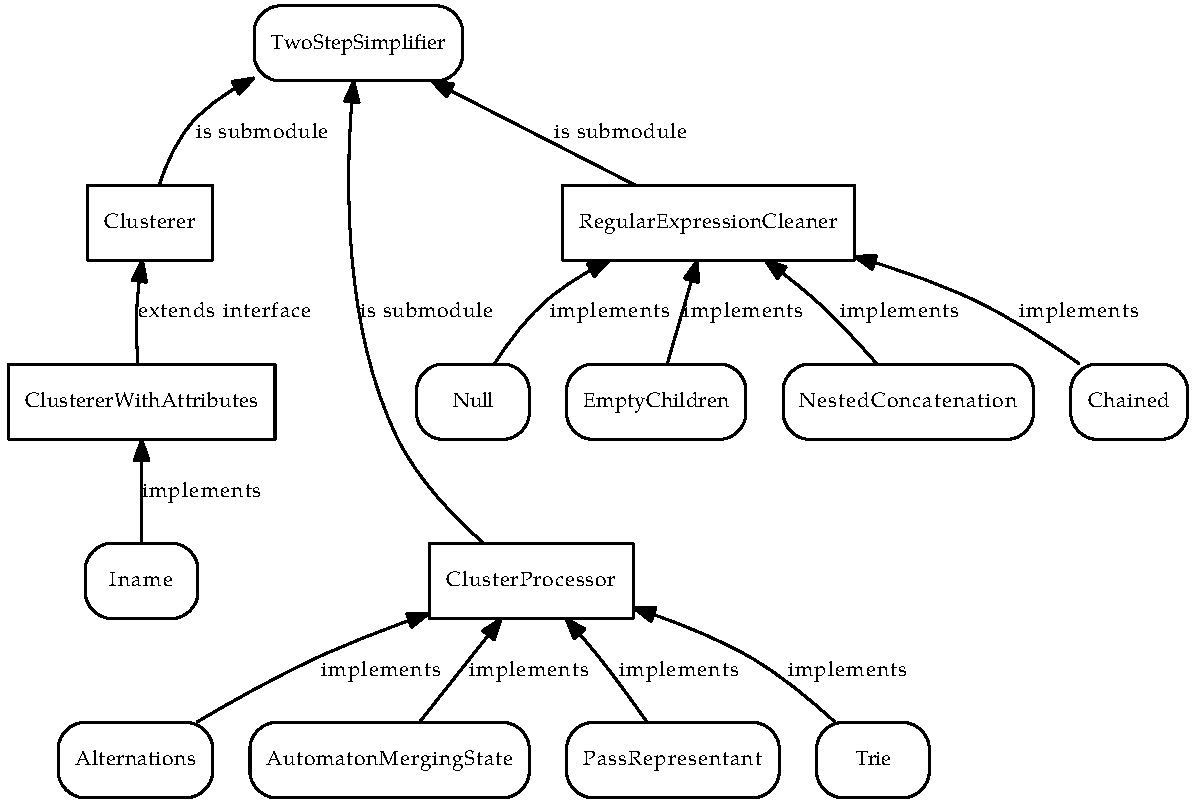
\includegraphics[scale=\myscale]{twostep_modules}
	\caption{Submodules of TwoStep simplifier with their implementations} \label{twostep_modules}
\end{figure}
We provide one \jmodule{Clusterer}, four \jmodule{ClusterProcessor} and four \jmodule{RegularExpressionCleaner} implementations.
Each of those will be explained further in this document.

Method \code{TwoStepSimplifier.simplify()} basically does the following.
\begin{verbatim}
// 1. cluster elements
Clusterer<AbstractStructuralNode> clusterer = clustererFactory.create();
clusterer.addAll(initialGrammar);
clusterer.cluster();

// 2. prepare emtpy simplified grammar
List<Element> simplifiedGrammar= new LinkedList<Element>();

// 3. process rules
ClusterProcessor<AbstractStructuralNode> processor =
             clusterProcessorFactory.create();
             
for (Cluster<AbstractStructuralNode> cluster : clusterer.getClusters()) {
  AbstractStructuralNode node =  
                          processor.processCluster(clusterer, cluster.getMembers());
  RegularExpressionCleaner<AbstractStructuralNode> cleaner = 
                          regularExpressionCleanerFactory.<AbstractStructuralNode>create();
  // 4. add to rules
  simplifiedGrammar.add(
              new Element(node.getContext(),
              node.getName(),
              node.getMetadata(),
              cleaner.cleanRegularExpression(((Element) node).getSubnodes()),
              attList));
}

return simplifiedGrammar;
\end{verbatim}
First, it creates a clusterer, gives it all the rules and performs the clustering.
Then, an empty list of elements is created as the simplified grammar.
For each input rule in \code{initialGrammar}, submodule \jmodule{ClusterProcessor} is invoked to infer the regular expression of that element.
Finally, regular expression cleaning is done by a submodule 
and new \code{Element} instance is created as a copy of processed node, but with inferred and cleaned regexp.

\paragraph{Sentinel processing}
There are some specialities in processing sentinel elements (see \cite[3.2]{archdoc}).
Sentinels can be only on the right side of rules. They have to be sent to clusterer, 
as someone further in the chain can ask for cluster of a sentinel element - which appears on right side.
However, sentinels have no content, and so they must not be taken into account when inferring attribute properties 
(whether it is required or optional), since sentinels have no attributes at all.

We will now examine the submodules for clustering, processing and cleaning.


%#### STRUCTURE->Clusterer ############################################
\subsection{Clusterer submodule}
Clustering is implemented in \code{cz.cuni.mff.ksi.jinfer.twostep.clustering} package.
One cluster is represented by the \code{Cluster<T>} class with \code{T} as type parameter of clustered items.
This class simply holds a \code{Set} of members of the cluster, one of which is chosen as a \code{representant}.

Any clusterer has to comply with the \code{Clusterer} interface.
Its purpose is to cluster a bunch of elements (rules) on input into a bunch of \code{Cluster} class instances (clusters) on output.
It has methods \code{add()} and \code{addAll()} for adding the input items to be clustered.
Main part is the method \code{cluster()}, which does the clustering itself.

As this may be a time-consuming operation, method throws \code{InterruptedException}.
Implementation should take care of checking whether thread is user interrupted (see \cite[p. 12]{archdoc}).
To be able to respond to calls to the \code{T getRepresentantForItem(T item)} method, 
every clusterer implementation has to keep all its clusters even after the clustering had finished. 
Using this method, given an item the correct cluster representative for this item has to be returned.

If no such cluster exists (item was not added for clustering before), we recommend throwing an exception rather than returning \code{null}.
Missing an item probably indicates error in the algorithm, rather than normal workflow.
One can get all the clusters (\code{List<Cluster<T>{}>}) from clusterer by calling \code{getClusters()} method.
Basic usage of the clusterer is:
\begin{verbatim}
Clusterer <T> c = new MyContextClusterer<T>();
c.addAll(initialGrammar);
c.cluster();
...
c.getClusters();
or
c.getRepresentantForItem(x);
\end{verbatim}

%#### STRUCTURE->Clusterer->WithAttributes ############################################
\subsubsection{ClustererWithAttributes extended interface}
You might have noticed that the \jmodule{Clusterer} interface and \code{Cluster} class are generic.
They may be used as design pattern not only for clustering elements in the inference process.
To address clustering of elements in more detail, we created \code{Cluster\.er\.With\.At\.tri\.bu\.tes<T, S>} interface, which extends \code{Clusterer<T>} interface.
It adds method \code{List\.<Cluster<S>{}> get\.At\.tri\.bu\.teClusters(T representant)}, implying that each representative of
type \code{T} (that is a representative of some main cluster) has some ``attribute'' clusters associated with it.
Attribute clusters are of type \code{S} and can be retrieved by calling \code{getAttributeClusters(x)}.

We provide one implementation of this interface described in \ref{section_Iname}.

%#### STRUCTURE->ClusterProcessor ############################################
\subsection{ClusterProcessor module}
\jmodule{ClusterProcessor} takes rules of one cluster of element and somehow obtains regular expression representing that set of elements. It returns one rule - element with name set to desired name of element in schema (not all elements in a cluster have to have same name, if advanced clustering scheme is used, then processor has to choose the right name for the resulting element) and with subnodes set to regular expression inferred.
It processes attributes of all elements in a cluster to obtain meaningful schema attribute specification. These attributes have to be attached to the resulting element.

Interface of submodule is defined as follows.
\begin{verbatim}
public interface ClusterProcessor<T> {
  T processCluster(
          Clusterer<T> clusterer,
          List<T> rules
          ) throws InterruptedException;
}
\end{verbatim}
Why is the cluster processor given a clusterer instance?
Rules themselves contain information about which elements to process, but clusterer has more information about the topic.
Clusterer can tell you the representative for any arbitrary element from input (not only those elements in rules, but also those that may be on right side of rules). Also, clusterer (if it is with attributes) has information about attributes in each cluster.

We describe each \jmodule{ClusterProcessor} implementation shipped in jInfer in sections \ref{section_PassRepresentant} through \ref{section_AutomatonMergingState}.

%#### STRUCTURE->RegularExpressionCleaner ############################################
\subsection{RegularExpressionCleaner module}
In this last subsection, we examine the \jmodule{RegularExpressionCleaner} interface.
Purpose of this submodule is only to make corrections to regular expression, to make them nicer on output.
For example, it is common that converting automaton to regular expression by state elimination produces nested concatenations such as $(name, (person, id))$.
To convert such expression into $(name, person, id)$, one can implement this interface and connect it to work in chain.
Interface definition is straightforward here.
\begin{verbatim}
public interface RegularExpressionCleaner<T> {
  Regexp<T> cleanRegularExpression(Regexp<T> regexp);
}
\end{verbatim}
Given a regular expression, return cleaned regular expression.
Conversion of regular expression is commonly a recursive task and all our implementations work this way.

%#### PREFERENCES ############################################
\section{Preferences}
All settings provided by \jmodule{TwoStepSimplifier} are project-wide, the preferences panel is in \code{cz.cuni.mff.ksi.jinfer.twostep.properties} package.
It is possible to set the following.
\begin{itemize}
	\item Select \jmodule{Clusterer} submodule implementation from those installed.
	\item Select \jmodule{ClusterProcessor} submodule implementation from those installed.
	\item Select \jmodule{RegularExpressionCleaner} submodule implementation from those installed.
\end{itemize}

%#### DATA FLOW ############################################
\section{Data flow}
\begin{figure}[tpb]
	\centering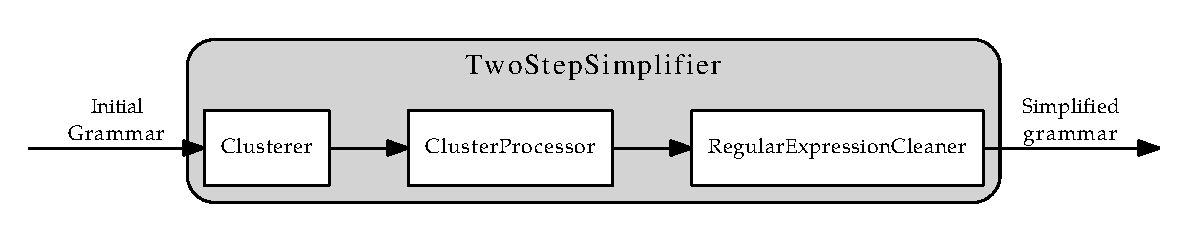
\includegraphics[scale=1]{twostep_flow}
	\caption{TwoStep data flow} \label{twostep_flow}
\end{figure}
Process illustrated in figure \ref{twostep_flow} is as follows.
\begin{enumerate}
	\item Initial Grammar on input, which is sent into \jmodule{Clusterer}.
	\item Each cluster is sent to submodule \jmodule{ClusterProcessor}, which returns regular expression for that cluster.
	\item Regular expression is sent to \jmodule{RegularExpressionCleaner} submodule for cleaning.
	\item Regular expressions representing all the processed clusters are added to the list of simplified grammar rules.
	\item List of simplified rules is returned (Simplified grammar).
\end{enumerate}

%#### SUBMODULES ############################################
\section{Submodule implementations}
%#### SUBMODULES->Iname ############################################
\subsection{Iname (ClusteterWithAttributes)} \label{section_Iname}
We cluster elements in \code{Iname\.<Abstract\.Structural\.Node, Attri\.bu\.te>} class, which takes \code{Abstract\.Structural\.No\.de} classes to cluster as main, and \code{Attribute} classes as attributes.
Clustering is done based on element's \code{getName()} equality (ignoring case).
For each rule (element), it is first clustered by finding the cluster which representative has the same name - or create new cluster with this element as representative.
Then we process right side of this element rule (that are nodes from \code{getSubnodes()}).
Since right side of rule is always concatenation (\jmodule{TwoStep} accepts only simple grammar representation), we simply take \code{.getSubnodes().getTokens()} list and iterate through it.
Each node on right side, is examined in the following way.
\begin{itemize}
  \item If it is \textbf{simple data}, throw it to \code{SimpleDataClusterer} class which is associated with main element cluster. It does nothing more, than holds all \code{SimpleData} instances in one cluster. But in future it may be replaced to cluster simple data somehow, to obtain meaningful content models in schemas.
  \item If it is \textbf{element} and it is tagged as sentinel - search main clusters to find cluster with representative of same \code{getName()}, or create new cluster with this sentinel as representative. From IGG, sentinels may be only on right sides of rules and since each element in schemas has to be defined, there must exist another element with same name, which is not sentinel (and maybe it will come to process in future). So there can't be cluster with only one sentinel element in it. 
  \item Do nothing otherwise, since it is element, it has to have its subnodes defined, and therefore it is element that is proper grammar rule and therefore it has to be somewhere in Initial Grammar, thus it is already processed or is on schedule.
\end{itemize}
Attributes of element are processed through a helper attribute clusterer, which is created for each element cluster.
We have bunch of elements of same name in a cluster and one attribute clusterer associated with this bunch.
This attribute clusterer is given all attributes instances encountered in all elements that are in bunch.
It clusters them by name, case insensitive.
Each main cluster also has \code{SimpleData} clusterer associated with it.
Whole scheme is on figure \ref{clusterer_structure}.
\begin{figure}[tpb]
	\centering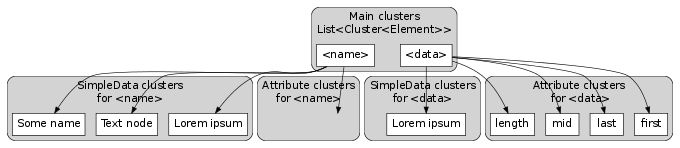
\includegraphics[scale=1]{clusterer_structure}
	\caption{Iname clusterer structure} \label{clusterer_structure}
\end{figure}

Once again, there are main clusters for elements, for each main cluster there are two helper clusterers - one for attribute clusters and one for simple data clusters.

%#### SUBMODULES->PassRepresentant ############################################
\subsection{PassRepresentant (ClusterProcessor)} \label{section_PassRepresentant}
Trivial ClusterProcessor implementation. For each cluster return its representative as the rule to be in resulting schema.
This has nothing to do with grammar simplification, it is just a proof-of-concept submodule.
Input documents are not valid against this odd grammar.
Do not use this in practice, just read the code to understand the bare minimum needed to implement a submodule.

%#### SUBMODULES->Alternations ############################################
\subsection{Alternations (ClusterProcessor)} \label{section_Alternations}
This processor simply gets all right sides from elements in cluster, puts them in one big list and creates alternation regular expression with this list as children.
That is, it creates one big rule with alternation of every positive example observed.
No generalization is done at all.

%#### SUBMODULES->Trie ############################################
\subsection{Trie (ClusterProcessor)} \label{section_Trie}
This processor takes all rules in a cluster, treats them like strings and builds a prefix tree (a ``trie'') of them. More precisely, it takes the first rule and declares it to be a long branch (concatenation of tokens) in a newly created tree. After that, it adds the remaining rules one by one as branches like this: as long as it can follow an existing branch, it follows it. As soon as the newly added branch starts to differ, it ``branches off'' (creates an alternation at that point) the existing tree and hangs the rest of the newly added rule there. Repeating this process creates a prefix tree describing all the rules in the cluster.
The tree is the final regular expression.

%#### SUBMODULES->AutomatonMergingState ############################################
\subsection{AutomatonMergingState (ClusterProcessor)} \label{section_AutomatonMergingState}
\begin{figure}[tpb]
	\centering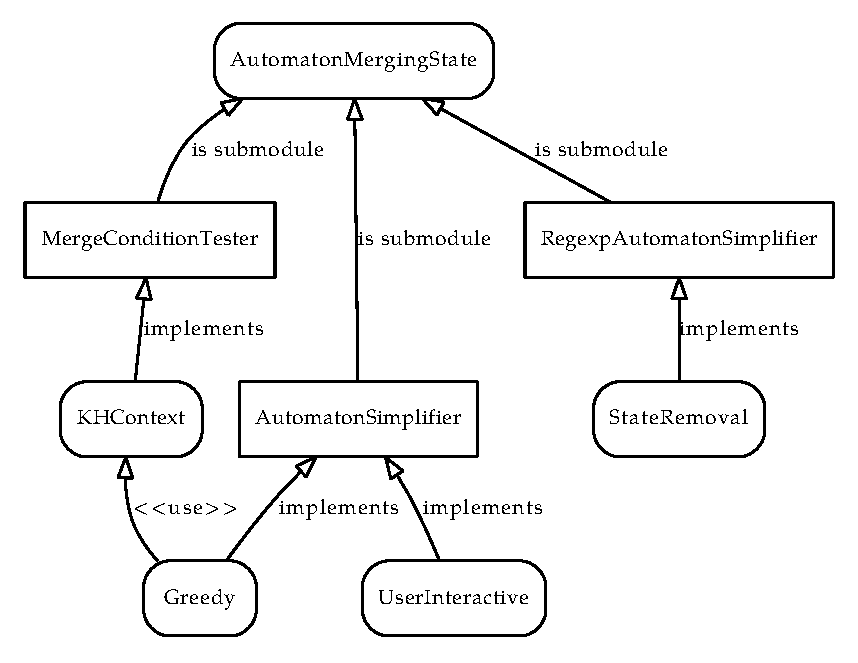
\includegraphics[scale=\myscale]{automaton_merging_state_modules}
	\caption{Submodules of AutomatonMergingState cluster processor} \label{automaton_merging_state_modules}
\end{figure}
\begin{figure}[tpb]
	\centering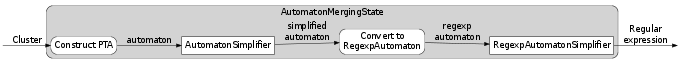
\includegraphics[scale=1]{automaton_merging_state_flow}
	\caption{Data flow of AutomatonMergingState cluster processor} \label{automaton_merging_state_flow}
\end{figure}
\jmodule{AutomatonMergingState} is an implementation of merging state algorithm on nondeterministic finite automaton (see package \code{cz.cuni.mff.ksi.jinfer.twostep.processing.automatonmergingstate}).
\subsubsection{Structure} \label{section_AutomatonMergingState_structure}
Abridged code of cluster processor operation follows.
\begin{verbatim}
// 1. Construct PTA
Automaton<AbstractStructuralNode> automaton = new Automaton<AbstractStructuralNode>(true);

// Take each rule in cluster and pass right side to automaton to create PTA
for (AbstractStructuralNode instance : rules) {
  Element element = (Element) instance;
  Regexp<AbstractStructuralNode> rightSide = element.getSubnodes();

  List<AbstractStructuralNode> rightSideTokens = rightSide.getTokens();

  List<AbstractStructuralNode> symbolString = new LinkedList<AbstractStructuralNode>();
  for (AbstractStructuralNode token : rightSideTokens) {
    symbolString.add(clusterer.getRepresentantForItem(token));
  }
  automaton.buildPTAOnSymbol(symbolString);
}

// 2. Simplify automaton by merging states using automatonSimplifier
Automaton<AbstractStructuralNode> simplifiedAutomaton =
    automatonSimplifier.simplify(automaton, elementSymbolToString);

// 3. Convert Automaton<AbstractStructuralNode> to RegexpAutomaton<AbstractStructuralNode>
RegexpAutomaton<AbstractStructuralNode> regexpAutomaton =
    new RegexpAutomaton<AbstractStructuralNode>(simplifiedAutomaton);
    
// 4. Call regexpAutomatonSimplifier to obtain regular expression from regexpAutomaton
Regexp<AbstractStructuralNode> regexp =
    regexpAutomatonSimplifier.simplify(regexpAutomaton, regexpAbstractToString);

// 5. Return element with regexp
return new Element(
      new ArrayList<String>(),
      rules.get(0).getName(),
      new HashMap<String, Object>(),
      regexp,
      new ArrayList<Attribute>()
      );
\end{verbatim}
The whole submodule structure is in figure \ref{automaton_merging_state_modules}.

\subsubsection{Data flow}
\jmodule{AutomatonMergingState} works in following steps.
\begin{enumerate}
	\item Create prefix-tree automaton (PTA) from positive examples - right sides of rules.
Call its submodule \jmodule{Au\.to\.ma\.ton\.Simpli\.fier} to modify PTA to some generalized automaton by merging states.
	\item Simplified automaton is then converted to an instance of \code{RegexpAutomaton} (see \ref{section_RegexpAutomaton}) by using clone constructor.
Regexp automaton is automaton with regular expression as symbol on transitions.
In automata theory, such automaton is called extended NFA.
Clone constructing is done by converting each symbol in source automaton to regexp token with that symbol as \code{content}.
	\item \code{RegexpAutomaton} is then passed into second submodule called \jmodule{RegexpAutomatonSimplifier}.
Its job is to derive regular expression from automaton, such that automaton and regular expression represent the same language.
\end{enumerate}
The data flow is depicted in figure \ref{automaton_merging_state_flow}.

\subsubsection{Data structures - Automaton} \label{section_Automaton}
\begin{figure}[tpb]
	\centering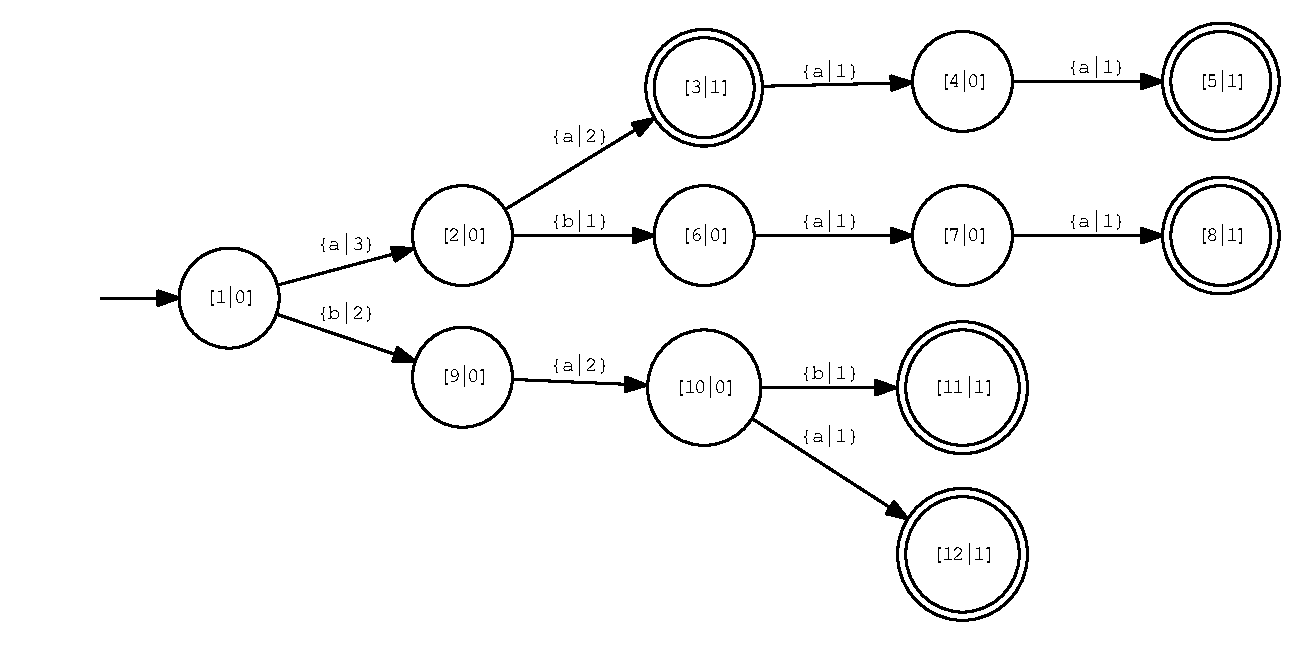
\includegraphics[scale=\myscale]{pta}
	\caption{PTA created from input strings: $aa, aaaaa, abaa, bab, baa$} \label{pta}
\end{figure}
Class \code{Automaton} is shortly described in \cite{archdoc}.
Let's take a look at method \code{build\.PTA\.On\.Sym\.bol} here.
Given \code{List<T> symbolString} it traverses automaton - comparing transition symbols with symbols in string.
It follows transitions in automaton until first difference with string symbol is found (like in prefix trees).
On different symbol, it creates new branch and all states and transitions on that branch.
Last state visited gets its \code{finalCount} value incremented, as one more input string ended in this state.
The code is as follows.
\begin{verbatim}
public void buildPTAOnSymbol(List<T> symbolString) {
  State<T> xState= this.getInitialState();
  for (T symbol : symbolString) {
    Step<T> xStep= this.getOutStepOnSymbol(xState, symbol);
    if (xStep != null) {
      xStep.incUseCount();
      xState= xStep.getDestination();
    } else {
      State<T> newState= this.createNewState();
      Step<T> newStep= this.createNewStep(symbol, xState, newState);
      assert newStep.getDestination().equals(newState);
      xState= newStep.getDestination();
    }
  }
  xState.incFinalCount();
}
\end{verbatim}
Starting from initial state, traverse the automaton by asking for \code{getOutStepOnSymbol()}.
If there is such step (transition), follow it to its destination state and move the position in \code{symbolString}.
If there is no such step, create one and create also the destination state, then follow this newly created step to new state.

As you can see, it is important that class \code{T} has proper implementation of \code{.equals()} method, as symbols are tested for equality by calling this method on them.
By the way, this is why we cluster all simple data and all sentinels on right sides of rules.	
While adding a concatenation to the automaton, instead of the instances themselves their \emph{representatives} are used. See \ref{section_AutomatonMergingState_structure} for further reference.
This assures that comparisons in automaton are done using Java \code{Object.equals()} reference comparison, but for each cluster member, its representative is only present in automaton.
That results in cluster-equal behaviour.
Example of prefix-tree automaton is in figure \ref{pta}.

\subsubsection{Data structures - RegexpAutomaton} \label{section_RegexpAutomaton}
Class \code{RegexpAutomaton} extends class \code{Automaton} with generic type \code{T} set to \code{Regexp<T>}.
That is, you have to instantiate it with same symbol type (e.g. \code{AbstractStructuralNode}) as automaton.
Implementation is in package \code{cz.cuni.mff.ksi.jinfer.twostep.processing.automatonmergingstate.regexping}. This is the same package where \jmodule{RegexpAutomatonSimplifier} interface is defined.
Implementation is nothing special - there is a copy constructor which creates regular expression automaton from ordinary automaton by enclosing each symbol on transition of original automaton in a \code{Regexp.TOKEN}.

\subsubsection{AutomatonSimplifier module}
\jmodule{AutomatonSimplifier} module has its worker interface defined as following.
\begin{verbatim}
public interface AutomatonSimplifier<T> {
  Automaton<T> simplify(Automaton<T> inputAutomaton, 
                        SymbolToString<T> symbolToString) throws InterruptedException;
  Automaton<T> simplify(Automaton<T> inputAutomaton, 
                        SymbolToString<T> symbolToString,
                        String elementName) throws InterruptedException;
}
\end{verbatim}
Given input automaton it returns automaton, there is nothing magical to it.
Interface is defined as generic, implementations don't have to be. However, there is no reason not to make them generic.
When implementation needs to present an automaton to user, it needs string representation of symbols to display on automaton transitions.
For this reason, the second parameter, \code{symbolToString} (implementation of \code{SymbolToString} interaface) is given.
It is responsible for converting symbol to string.
Overloaded version is to inform the user about name of processed element when presenting automaton in \jmodule{AutoEditor}.
This version of interface will probably change in future.

This generality means that simplifier can not only be used to infer rules for elements, but possibly also to infer patterns strings for content model of attributes using the same algorithms.
The actual implementation of this still waits for its developer to come.
Implementations of \jmodule{AutomatonSimplifier} are discussed in \ref{section_Greedy} and \ref{section_UserInteractive}.

\subsubsection{RegexpAutomatonSimplifier submodule}
Purpose of \jmodule{RegexpAutomatonSimplifier} is to obtain a regular expression from a given automaton.
Interface for doing is is thus simple.
\begin{verbatim}
public interface RegexpAutomatonSimplifier<T> {
  Regexp<T> simplify(RegexpAutomaton<T> inputAutomaton, 
                     SymbolToString<Regexp<T>> symbolToString) throws InterruptedException;
}
\end{verbatim}
Once again we encounter \code{symbolToString} with the same purpose as before, if submodule would need to present the automaton to user, it has to be able to convert symbols of (at runtime) unknown type to strings.
Our implementation of \jmodule{RegexpAutomatonSimplifier} is discussed in \ref{section_StateRemoval}

\subsubsection{MergeConditionTester submodule}
\jmodule{AutomatonMergingState} has one more submodule, the \jmodule{MergeConditionTester}, which is not called directly by \jmodule{Au\.to\.ma\.ton\.Merg\.ing\.Sta\.te}.
It is at disposal of implementations of \code{AutomatonSimplifier} interface for testing, whether two states in automaton are equivalent and should be merged into one state.

One can implement ACO heuristics or MDL principle heuristics as \jmodule{AutomatonSimplifier} submodule, and can use any of \jmodule{MergeConditionTesters} provided.

\subsection{NestedConcatention (RegularExpressionCleaner)} \label{section_NestedConcatention}
It converts nested concatenations into flat ones.
Example: $(name, (person, id))$ is converted to $(name, person, id)$.

\subsection{Null (RegularExpressionCleaner)} \label{section_Null}
This cleaner just returns regexp it receives and does nothing.
Plug this one into chain, if you want to omit this step in inference.

\subsection{EmptyChildren (RegularExpressionCleaner)} \label{section_EmptyChildren}
Wipes out regular expressions of type: concatenation, alternation, permutation, which have empty \code{children} member.
If for example an inference method produces unnecessary empty regexps in regexp tree such as
$$
(name, (), (person, id))
$$
There is one empty concatenation/alternation/permutation with no sense.
This is wiped out by this cleaner to produce 
$$
(name, (person, id))
$$

\subsection{Chained (RegularExpressionCleaner)} \label{section_Chained}
Allows the user to chain more cleaners with output from first one plugged as input into second one and so one.
Thus regular expression from inference can pass through \jmodule{EmptyChildren} and then through \jmodule{NestedConcatenation} cleaners and then it is returned.

\subsection{Greedy (AutomatonSimplifier)} \label{section_Greedy}
We implement greedy strategy of automaton simplifying in class \code{Greedy}.
It simply asks given \code{MergeConditionTester} if it can merge any of automaton states and merges states until there are no states to be merged.
\begin{verbatim}
while (there exist pair of states that are equivalent) {
  merge them
}
\end{verbatim}
We provide one \jmodule{MergeConditionTester} implementation, see \ref{section_KHContext}.

\subsection{UserInteractive (AutomatonSimplifier)} \label{section_UserInteractive}
We have created automaton simplifier which shows the user the input automaton, asking him to select states to merge.
Then it merges them and asks user again.
\begin{verbatim}
repeat {
  draw automaton
  if (user selects more than one state to merge) {
    merge them
  }
} until (user selected at least one state in last attempt)
\end{verbatim} 
We use \jmodule{AutoEditor} module described in \cite{autoeditordoc}.
A screenshot of automaton visualization is in picture \ref{screenshot}.
\begin{figure}[tpb]
	\centering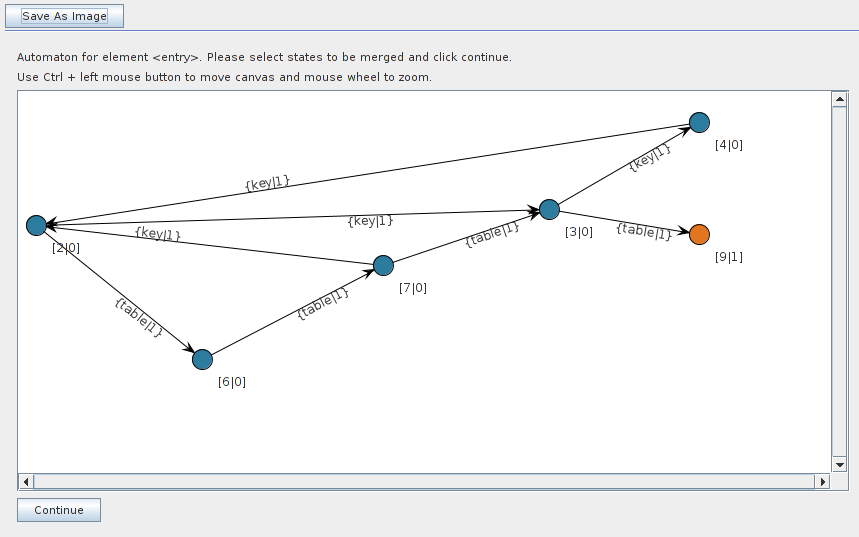
\includegraphics[scale=0.5]{screenshot}
	\caption{Screenshot of UserInteractive (AutomatonSimplifier).} \label{screenshot}
\end{figure}

\subsection{KHContext (MergeConditionTester)} \label{section_KHContext}
We have implemented \emph{k,h-context} state equivalence (see \cite{ahonen}) in class \code{KHContext} (implements \code{Mer\.ge\.Con\.di\.tion\.Tes\.ter} interface), which is used by \code{Greedy} to test mergeability of states.
We don't use $k-grams$ algorithm from \cite{ahonen}, just a simple DFS.

\subsection{StateRemoval (RegexpAutomatonSimplifier)} \label{section_StateRemoval}
\begin{wrapfigure}{R}{40mm}
	\centering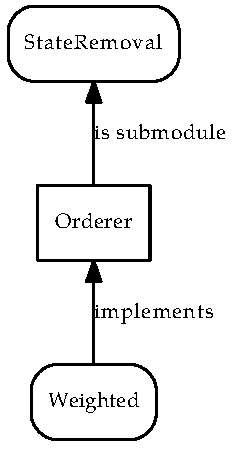
\includegraphics[scale=\myscale]{state_removal_modules}
	\caption{Modules of StateRemoval.} \label{state_removal_modules}
	\vspace{10mm}
\end{wrapfigure}
We are using state removal method (see \cite{1224321}) to convert regexp automaton into equivalent regular expression.
This is implemented in \code{StateRemoval} class (figure \ref{state_removal_modules}) which implements \code{RegexpAutomatonSimplifier} interface.
Before the algorithm starts, states \emph{superInitial} and \emph{superFinal} are added to automaton, former with $\lambda$-transition to initial state.
From all final states a $\lambda$ transition to \emph{superFinal} state is added.
State removal works by removing states of automaton (and redirecting transitions properly) until there are last to two states - \emph{superInitial} and \emph{superFinal}.
After removing all states, there is only one transition from \emph{superInitial} to \emph{superFinal} state.
That transition has the final regular expression as symbol on it. This one is returned.

We defined one submodule of this class with \jmodule{Orderer}.
It has only one method to implement: \code{getStateToRemove}.
Given automaton, it has to return reference to one state which should be removed from automaton at first.
State removal calls this submodule and removes state returned.

\subsubsection{Data Structures - StateRemovalRegexpAutomaton}
We extend \code{RegexpAutomaton} to obtain automaton that fits the state removal procedure.
This implementation has methods \code{crea\.te\.Su\.per\.In\.it\.ial\.Sta\.te} and \code{crea\.te\.Su\.per\.In\.it\.ial\.Sta\.te}.
They does exactly what their names stands for.
\emph{SuperInitial} state has only one $\lambda$-out-transition pointing to original initial state.
\emph{SuperFinal} state has as many $\lambda$-in-transitions, as there are original final states - from each one it gets one.
Without going further into many technical details, we just mention method \code{removeState}, which removes given state from automaton.
Transitions are handled in the following way.
\begin{enumerate}
	\item Collapse all loop transitions of removed state to one loop transition with new \code{Regex.ALTERNATION} of all regexps on original loops (with Kleene interval set).
	\item Collapse all {in | out}-transitions, which same {source | destination} state to one transition with \code{Reg\.exp.AL\.TER\.NA\.TION} of original regexps.
	\item For each in-transition, loop, and out-transition, add transition from in-transition source to out-transition destination with symbol of \code{Regexp.CONCATENATION} of in-transition regexp, loop regexp and out-transition regexp. Thus by-passing the state completely.
	\item Remove the state and transitions associated with it.
\end{enumerate}
The whole process is step-by-step illustrated in figure \ref{regaut}.
\begin{figure}[pb]
	\centering
	\subfigure[RegexpAutomaton after conversion from ordinary automaton.]
	{
		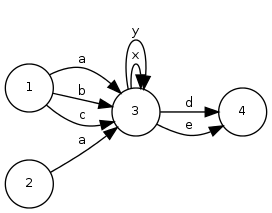
\includegraphics[scale=\myscale]{regaut1}
		\label{regaut1}
	}
	\subfigure[First, collapse loop transitions to alternation with Kleene interval set.]
	{
		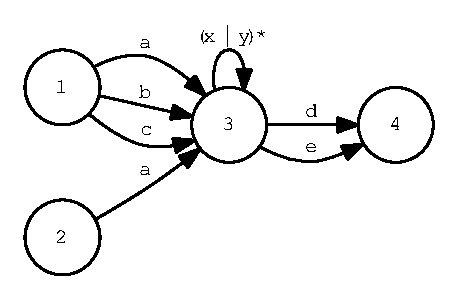
\includegraphics[scale=\myscale]{regaut2}
		\label{regaut2}
	}
	\subfigure[Collapse {in | out}-transitions {from | to} same states.]
	{
		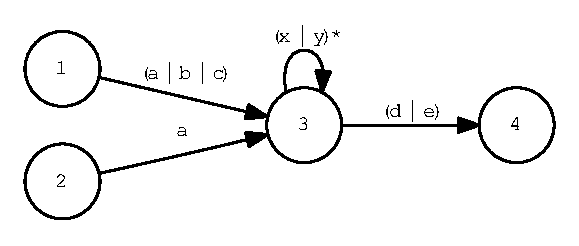
\includegraphics[scale=\myscale]{regaut3}
		\label{regaut3}
	}
	\subfigure[Bypass state 3 by adding concatenation transitions from states 1 and 2 to state 4. Remove state 3 and associated transitions.]
	{
		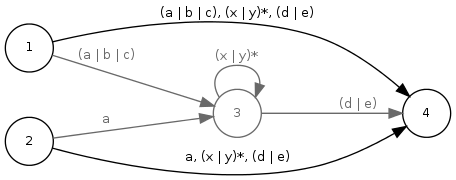
\includegraphics[scale=\myscale]{regaut4}
		\label{regaut4}
	}
%	
%	\subfigure[Finally remove state 3 and associated transitions.]
%	{
%		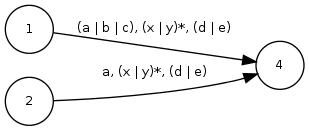
\includegraphics[scale=\myscale]{regaut5}
%		\label{regaut5}
%	}
	\caption{RegexpAutomaton and removing state 3 from it.} \label{regaut}
\end{figure}

\subsection{Weighted (Orderer)} \label{section_Weighted}
We implement one orderer, called \code{Weighted}.
It is simple heuristic - weights all states (weight = sum of {in | out | loop}-transition regular expression lengths) and returns state with lowest weight.

%#### EXTENSIBILITY ############################################
\section{Extensibility}
If you are willing to, you can replace each of three submodules of \jmodule{TwoStepSimplifier}.
It may be useful to replace the default \jmodule{ClustererWithAttributes} implementation with a clever one.
And regular expression cleaning will be probably the aim of new implementations, too.
We recommend replacing other parts at lower levels, however.
You will need to replace \jmodule{ClusterProcessor} only if you want to write inference method that is not based on merging state algorithm (or NFA's at all).

If this is not your case, you can replace module \jmodule{AutomatonSimplifier} to implement ACO heuristics or MDL principle in searching solutions of merging states.

Of course, merge criterion is probably the point to add implementation, implement \jmodule{MergeConditionTester} interface to obtain for example $s,k$-string merge criterion.

Changing ordering of states to remove in \jmodule{StateRemoval} module is easy by replacing \jmodule{Orderer} implementation, for example to one suggested in \cite{1224321} may lead to shorter resulting regular expressions.

Whole TwoStep submodules structure is in figure \ref{twostep_modules_complete}.
\begin{figure}[tpb]
	\centering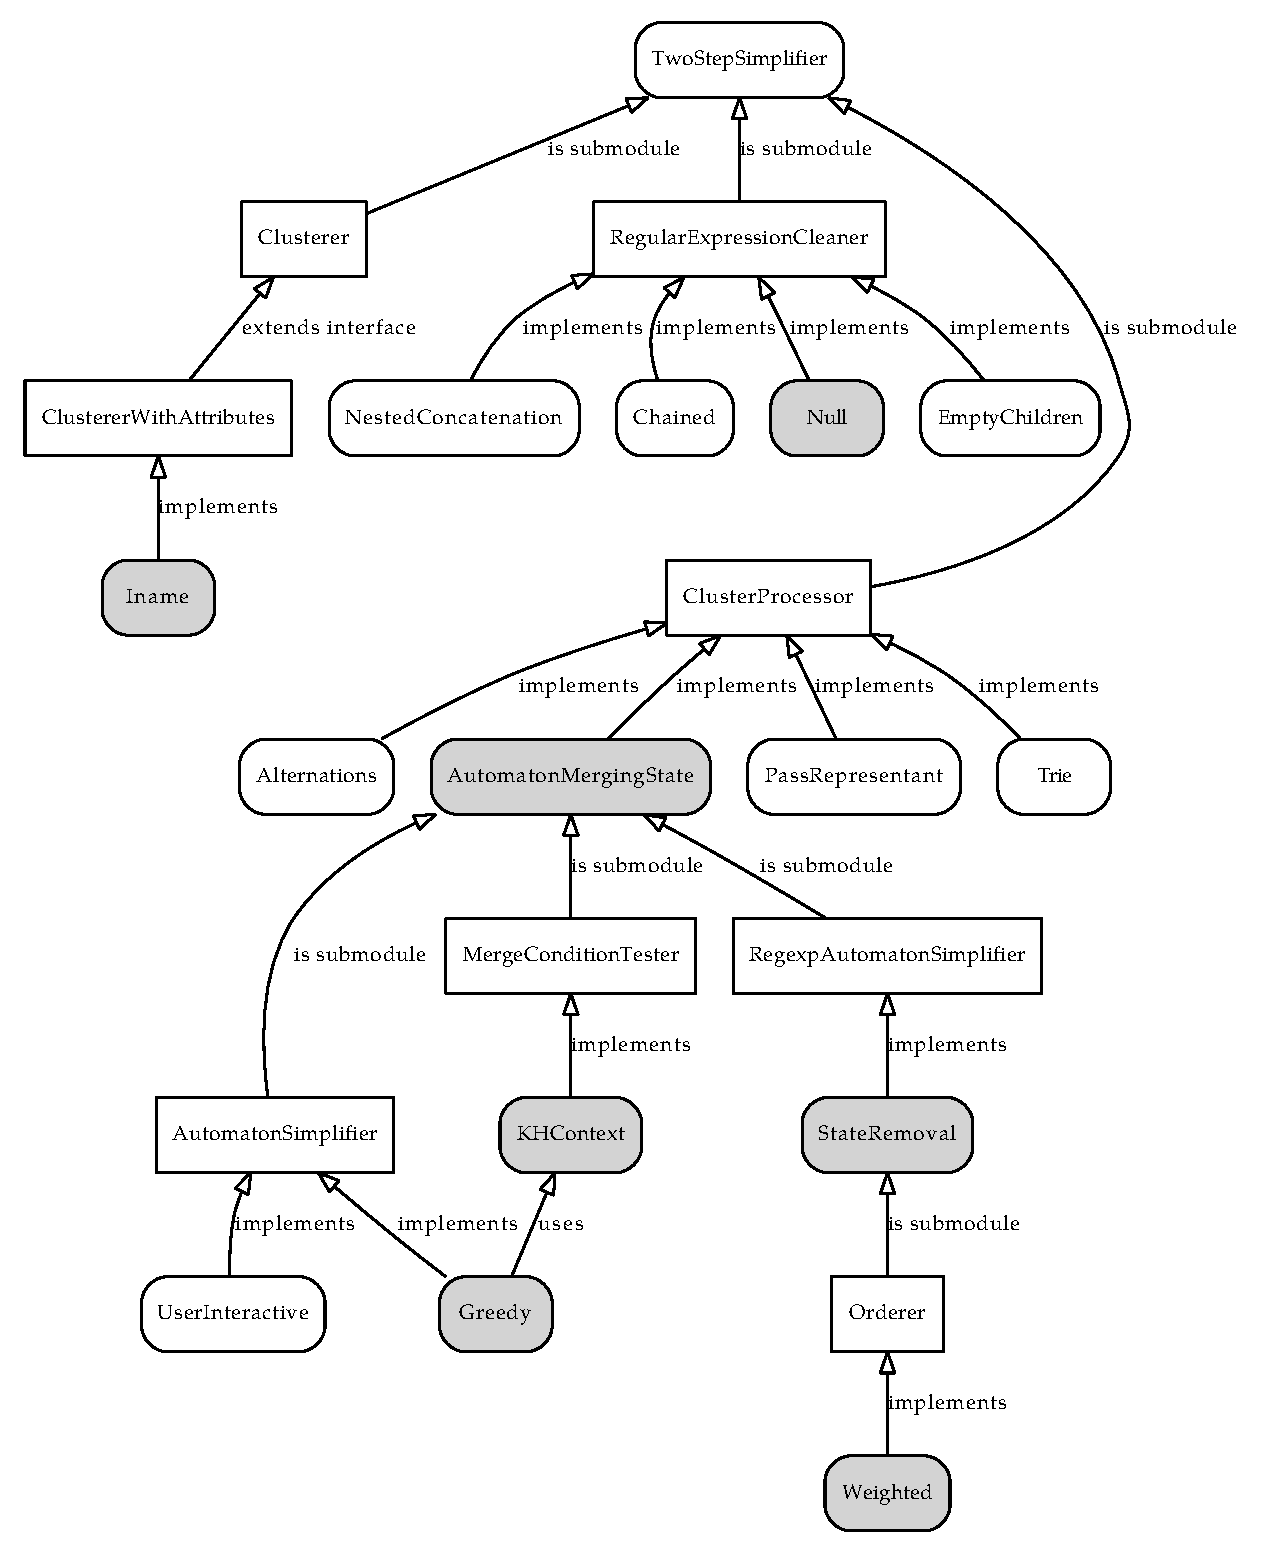
\includegraphics[scale=0.37]{twostep_modules_complete}
	\caption{Modules of TwoStep simplifier and their submodules. Filled classes are default selection (best of).} \label{twostep_modules_complete}
\end{figure}

\nocite{*}
\newpage
\bibliographystyle{alpha}
\bibliography{literature}

\end{document}
